\documentclass[xcolor=pdftex,dvipsnames]{beamer}

\usepackage{amsmath}
\usepackage{amssymb}
\usepackage{comment}
\usepackage{textcomp}
\usepackage{ulem}
\DeclareRobustCommand{\rsout}[1]{\texorpdfstring{\sout{#1}}}

\title{Microeconomic Theory --- ECON 323 503 \\ Chapter 14: Oligopoly
 \rsout{and Monopolistic Competitions}}
\author{Vikram Manjunath}       %
\institute{Texas A\&M University}
\setbeamertemplate{navigation symbols}{}
\setbeamertemplate{footline}{}
\usefonttheme{serif}
\begin{document}

\maketitle

\begin{frame}
\frametitle{Outline}
\begin{enumerate}[<+->]
\item The Cournot oligopoly model: two (or more) firms simultaneously
  pick quantities to produces.
\item The Stackelberg oligopoly model: two firms pick quantities one after another.
\item The Bertrand oligopoly model: two (or more) firms simultaneously
  pick prices.
\end{enumerate}
\end{frame}


\begin{frame}
  \frametitle{The Cournot oligopoly model}
  Remember the airline example.
  \bigskip
  
\uncover<2->{  We'll expand this in two ways:}
  \begin{enumerate}
  \item<3-> Any quantity is possible (not just 48, 64, or 96).
  \item<4-> There are $n$ airlines, not just 2.
  \end{enumerate}

\end{frame}

\begin{frame}
  \frametitle{Any quantity}
  The total quantity ($Q = q_A  + q_U$) affects the price.
\bigskip

\uncover<2->{  This relationship is given by the inverse demand function:
\[
p = 339 -Q
\]}

\uncover<3->{  Costs factor into the decisions of $U$ and $A$ as well.}
\bigskip

\uncover<4->{  Assume constant $MC$ of \$147 and no fixed cost so that $AC = MC$.}

\end{frame}

\begin{frame}
  \frametitle{Monopoly for comparison}
  If $A$ were a monopoly, $MR_A = 339 - 2{q_A}.$

\bigskip
\uncover<2->{  Monopoly quantity would be 96 (from $MR_A = MC = 147$).}
\uncover<3->{  \begin{center}
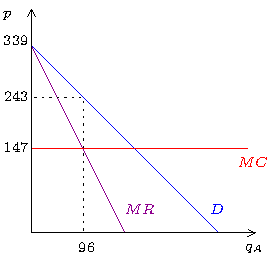
\includegraphics{pics/MonopolyAirline}
\end{center}}
\end{frame}


\begin{frame}
  \frametitle{When there are two firms}
If $U$ produces $q_U$, what is the inverse demand function that $A$ faces?

\uncover<2->{  \[
p =  339 - Q = 339 - (q_A+q_U) = (339 - q_U) - q_A.
\]}

\uncover<3->{  If $A$ picks $q_A$, what is its revenue?}

\uncover<4->{  \[
\begin{array}{rcl}
  R_A(q_A)& =& pq_A\\\\
&=& ((339 - q_U) - q_A)q_A\\\\
&=& 339q_A - q_Uq_A - q_A^2.
\end{array}
\]}


\end{frame}
\begin{frame}
  \frametitle{$A$'s decision}
  To know what $A$ will do, we just set $MR_A=MC$.

\uncover<2->{  \[
MR_A = \frac{dR_A(q_A)}{d q_A}  = 339 - q_U -2q_A.
\]}

\uncover<3->{  Equating this with $MC$:
\[
339 - q_U - 2q_A = 147
\]}
\uncover<4->{  Solving for $q_A$:
\[
q_A = 96 - \frac{1}{2}q_U.
\]}

\uncover<5->{  So $A$'s \textit{best response} to $U$'s choice of $q_U$ is
\[
B_A(q_U) = 96 - \frac{1}{2}q_U.
\]
}
\end{frame}

\begin{frame}
  \frametitle{$A$'s best response }
  \begin{center}
    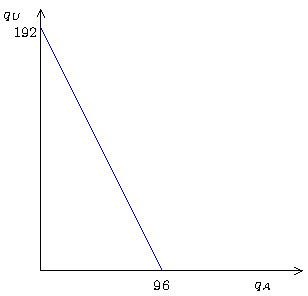
\includegraphics{pics/Cournot1}
  \end{center}
If $U$ doesn't produce anything, $A$ picks 96. If $U$ produces 192 or
more, $A$'s best response is to shut down.
\end{frame}

\begin{frame}
  \frametitle{$U$'s best response}
  The two firms are identical. \uncover<2->{  So $U$'s best response to $A$'s choice
  fo $q_A$ is
\[
B_U(q_A) = 96 - \frac{1}{2}q_A.
\]}





\end{frame}

\begin{frame}
  \frametitle{Nash-Cournot equilibrium}
  Remember that a Nash equilibrium is where each player is best
responding to the other's strategy.

\bigskip
\uncover<2->{  $U$ choosing $q_U$ and $A$ choosing $q_A$ is a Nash equilibrium
of the ``Cournot game'' when 
\[
q_A = B_A(q_U)\text{ and }q_U = B_U(q_A).
\]}

\uncover<3->{  So
\[
q_A = 96 - \frac{1}{2}q_U \text{ and  } q_B  = 96 - \frac{1}{2}q_A.
\]}

\uncover<4->{  Solving for $q_A$ and $q_U$,
\[
q_A = q_U = 64.
\]}


\end{frame}

\begin{frame}
  \frametitle{Graphically}
  \begin{center}
    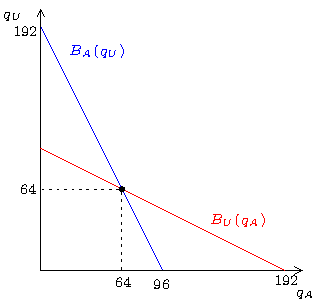
\includegraphics{pics/Cournot2} 
  \end{center}
\end{frame}

\begin{frame}
  \frametitle{With many firms}
  If there are $n$ firms producing $q_1, q_2, \dots, q_n$:
\[
Q = q_1+ q_2 + \dots + q_n
\]
\uncover<2->{  And 
\[
p = p(Q).
\]}

\uncover<3->{  Cost for firm $i$ is $C(q_i)$. }


\end{frame}

\begin{frame}
  \frametitle{Many firms}
  What will each firm do? 

\bigskip
\uncover<2->{  Start with firm 1's decision. Its profit is (when production decisions
are $q_1, \dots, q_n$)
\[
\pi_1 (q_1, \dots ,q_n) = q_1p(Q) - C(q_1)
\]}
\uncover<3->{  Firm 1's first order condition:
\[
\frac{\delta \pi}{\delta q_1} = p(Q) + q_1
  \frac{dp(Q)}{dQ}\frac{\delta Q}{\delta q_1} -
  \frac{dC(q_1)}{dq_1}= 0
\]}
\uncover<4->{  This is just 
\[
MR = p(Q) + q_1
  \frac{dp(Q)}{dQ} =   \frac{dC(q_1)}{dq_1}= MC
\]}
\uncover<5->{  Firm 1's \textit{best response} to the other firms' choices is to pick
$q_1$ that solves this equation.}

\end{frame}
\begin{frame}
  \frametitle{Many firms}
Solving that $n$ equations, one for each firm, we end up with $q_1$
through $q_n$ which constitute a Nash equilibrium.

\bigskip
\uncover<2->{    Since the firms are all identical these equations are identical.}

\bigskip
\uncover<3->{  So, in equilibrium $q_1 = q_2 = \dots = q_n$.}

\bigskip
\uncover<4->{  We'll just call this common choice by all of the firms $q$}

\bigskip
\uncover<5->{  Since there are $n$ firms, $Q = nq$.}




\end{frame}

\begin{frame}
  \frametitle{How far from competitive?}
Let's mess MR a little so that we can figure out the ratio $\frac{p}{MC}$.
  \[
  \begin{array}{rcl}
    MR &  = &p + q   \frac{dp}{dQ}\\\\
\uncover<2->{&=& p + \frac{1}{n} nq \frac{dp}{dQ}\\\\}
\uncover<3->{&=& p + p\frac{1}{n} \frac{Q}{p} \frac{dp}{dQ}\\\\}
\uncover<4->{&=& p\left[1 + \frac{1}{n} \frac{Q}{p} \frac{dp}{dQ}\right]\\\\}
\uncover<5->{&=& p\left[1+\frac{1}{n\varepsilon}\right].}
  \end{array}
\]
\end{frame}
\begin{frame}
  \frametitle{Price/cost ratio}
  Now, setting $MR = MC$ is
\[
p\left[1+\frac{1}{n\varepsilon}\right] = MC
\]
\uncover<2->{ So
\[
p = \frac{MC}{\left[1+\frac{1}{n\varepsilon}\right]}.
\]}
\uncover<3->{ Or 
\[
\frac{p}{MC} = \frac{1}{\left[1+\frac{1}{n\varepsilon}\right]}.
\]}

\end{frame}
\begin{frame}
  \frametitle{Lerner index}
  How far are we from the competitive market outcome?

\bigskip
\uncover<2->{ The Lerner index is a measure of this:}
\[
\begin{array}{rcl}
\uncover<3->{\frac{p-MC}{p} &=& 1-   \frac{MC}{p}\\\\}
\uncover<4->{ &=& 1-   \left[1+\frac{1}{n\varepsilon}\right]\\\\}
\uncover<5->{& = & -\frac{1}{n\varepsilon}}
\end{array}
\]
\uncover<6->{ As the number of firms grows, this gets closer to zero.}
\bigskip

\uncover<7->{ So as the number of firms in the Bertrand game, the closer we get to
the competitive outcome.}

\end{frame}


\begin{frame}
  \frametitle{Linear case}
  We don't have a nice formula for $q$ without specifying $C$ and $p$.
\bigskip

\uncover<2->{ Assume constant marginal cost (with no fixed cost) of $m$ (so $C(q) = mq$.)}

\bigskip
\uncover<3->{ Let
\[
p = a-bQ.
\]}

\uncover<4->{ Then 
\[MR = a - b(2q_1 + q_2 + \dots q_n) = m = MC\]}

\uncover<5->{ If $q_2 = q_3 = \dots = q_n = q$, then
\[q_1 = B_1(q_2,\dots, q_n) = \frac{a-m}{2b} - \frac{n-1}{2}q.\]}


\end{frame}
\begin{frame}
  \frametitle{Linear case}
Since $q_1= q$ in equilibrium,
\[
q = \frac{a-m}{2b} - \frac{n-1}{2}q.
\]
\uncover<2->{  Solving this, in equilibrium each firm picks,
\[
q = \frac{a-m}{(n+1)b}.
\]}

\uncover<3->{ So the equilibrium price is 
\[
p = \frac{a+nm}{n+1}
\]}

\uncover<4->{ When $n=1$ these are the monopoly quantity and price.}
\bigskip

\uncover<5->{ As $n$ grows larger, these get closer to the competitive quantity and price.}



\end{frame}

\begin{frame}
  \frametitle{The airline game}
  We can figure out what happens if there are $n$ airlines:

\uncover<2->{\[
\begin{array}{rcl}
  a & = & 339\\
b &=& 1\\
m&=& 147
\end{array}
\]}

\uncover<3->{ Using what we solved earlier
\[
q = \frac{339 -147}{n+1}\text{ and }p = \frac{339 + 147 n}{n+1}.
\]}
\uncover<4->{ Check that if $n=1$ we get the monopoly price/quantity and if $n=2$ we
get the duopoly price/quantity.}

\end{frame}

\begin{frame}
  \frametitle{The Stackelberg oligopoly model}
  $A$ picks a quantity first and then $U$ gets to pick.
\bigskip

\uncover<2->{ If $A$ has chosen $q_A$, we already figured out what $U$ will do:
\[q_U = B_U(q_A)  = 96 - \frac{1}{2}q_A\]}
\bigskip

\uncover<3->{ What should $A$ choose?}
\bigskip

\uncover<4->{$A$ wants to maximize
\[
\begin{array}{rcl}
\pi_A(q_A) &=& p(q_A + q_U)q_A - C(q_A)  \\\\}
\uncover<5->{&=& p(q_A+ (96 - \frac{1}{2}q_A))q_A - mq_A\\\\}
\uncover<6->{&=& (339 - 96 - \frac{1}{2}q_A)q_A - 147q_A\\\\}
\uncover<7->{&=& 96q_A - \frac{1}{2}q_A^2.}
\end{array}
\]


\end{frame}


\begin{frame}
  \frametitle{$A$'s choice}
  \[
  \begin{array}{rcl}
\frac{d\pi_A}{dq_A} &=& 0\\\\
\uncover<2->{\frac{d\left(96q_A - \frac{1}{2}q_A^2\right)}{dq_A} &=& 0\\}
\uncover<3->{ 96 - q_A & =& 0\\\\}
\uncover<4->{ q_A & = & 96.}
  \end{array}
\]
\uncover<5->{ So, 
\[q_U = B_U(q_A)} \uncover<6->{ = 96 - \frac{1}{2} q_A}\uncover<7->{ = 96 - \frac{1}{2}96}\uncover<8->{ = 48.\]}


\end{frame}



\begin{frame}
  \frametitle{The Bertrand oligopoly model}
  What if firms pick prices rather than quantity?
  
  \bigskip
\uncover<2->{  If firm 1's price is lower than firm 2's price: all consumers buy
  only from firm 1.}

  \bigskip
\uncover<3->{  If firm 1's price is higher than firm 2's price: all consumers buy
  only from firm 2.}

  \bigskip
\uncover<4->{  Assume that MC is constant ($MC = \$5$)}

\end{frame}

\begin{frame}
  \frametitle{Nash-Bertrand Equilibrium}
  What happens if firm 1 charges \$10?

  \bigskip
\uncover<2->{  Firm 2 could capture the entire market by charging \$9.99.}

  \bigskip
\uncover<3->{  But if firm 2 charges \$9.99, firm 1 would charge \$9.98.}
\bigskip

\uncover<4->{\dots}
\bigskip

\uncover<5->{ If firm 1 charges \$5.01, firm 2 would charge \$5.005}
\bigskip

\uncover<6->{\dots}

\bigskip
\uncover<7->{ Unless a firm charges \$$5=MC$, the other would under cut it.}

\bigskip
\uncover<8->{ Caveat: this reasoning relies on firms beign able to produce any quantity.}
\end{frame}


\begin{frame}
  \frametitle{Do we only need two firms for profits to disappear?}
  Which is more realistic: Bertrand or Cournot?


\bigskip
\uncover<2->{ If $\varepsilon = -1$ the Cournot price would be
\$10 ($=\frac{MC}{1+\frac{1}{2\varepsilon}} = \frac{5}{1-\frac{1}{2}}$)}

\bigskip
\uncover<3->{ Which is a more reasonable price to expect: \$5 or \$10?}

\bigskip
\uncover<4->{ The Cournot model is more plausible for two reasons:}
\begin{enumerate}
\item<5-> Observed oligopoly prices are typically, like the Cournot
  price, between the competitive price  and the monopoly price.
\item<6-> The Bertrand price only depends on cost and is completely
  independent of demand. But observations are that prices vary with demand.
\end{enumerate}

\end{frame}

\end{document}



